\documentclass[a4paper,11pt,fleqn,dvipsnames,twoside,openany]{memoir} 	% Openright aabner kapitler paa hoejresider (openany begge)

%%%% PACKAGES %%%%

% ¤¤ Oversaettelse og tegnsaetning ¤¤ %
\usepackage[utf8]{inputenc}					% Input-indkodning af tegnsaet (UTF8)
\usepackage[english]{babel}					% Dokumentets sprog
\usepackage[T1]{fontenc}					% Output-indkodning af tegnsaet (T1)
\usepackage{ragged2e,anyfontsize}			% Justering af elementer
\usepackage{fixltx2e}						% Retter forskellige fejl i LaTeX-kernen
																			
% ¤¤ Figurer og tabeller (floats) ¤¤ %
\usepackage{caption}
\usepackage{subcaption}
\usepackage{graphicx} 						% Haandtering af eksterne billeder (JPG, PNG, EPS, PDF)
%\usepackage{eso-pic}						% Tilfoej billedekommandoer paa hver side
%\usepackage{wrapfig}						% Indsaettelse af figurer omsvoebt af tekst. \begin{wrapfigure}{Placering}{Stoerrelse}
\usepackage{multirow}                		% Fletning af raekker og kolonner (\multicolumn og \multirow)
\usepackage{multicol}         	        	% Muliggoer output i spalter
\usepackage{rotating}						% Rotation af tekst med \begin{sideways}...\end{sideways}
\usepackage{colortbl} 						% Farver i tabeller (fx \columncolor og \rowcolor)
\usepackage[table]{xcolor}				 	% Definer farver med \definecolor. Se mere: http://en.wikibooks.org/wiki/LaTeX/Colors
\usepackage{flafter}						% Soerger for at floats ikke optraeder i teksten foer deres reference
\let\newfloat\relax 						% Justering mellem float-pakken og memoir
\usepackage{float}							% Muliggoer eksakt placering af floats, f.eks. \begin{figure}[H]
\usepackage{wrapfig}



% ¤¤ Matematik mm. ¤¤
\usepackage{amsmath,amssymb,stmaryrd} 		% Avancerede matematik-udvidelser
\usepackage{mathtools}						% Andre matematik- og tegnudvidelser
\usepackage{textcomp}                 		% Symbol-udvidelser (f.eks. promille-tegn med \textperthousand )
\usepackage{rsphrase}						% Kemi-pakke til RS-saetninger, f.eks. \rsphrase{R1}
\usepackage[version=3]{mhchem} 				% Kemi-pakke til flot og let notation af formler, f.eks. \ce{Fe2O3}
\usepackage{siunitx}						% Flot og konsistent praesentation af tal og enheder med \si{enhed} og \SI{tal}{enhed}
\sisetup{locale=DE}							% Opsaetning af \SI (DE for komma som decimalseparator) 

% ¤¤ Referencer og kilder ¤¤ %
\usepackage[danish]{varioref}				% Muliggoer bl.a. krydshenvisninger med sidetal (\vref)
\usepackage[square,sort,comma,numbers]{natbib}							% Udvidelse med naturvidenskabelige citationsmodeller
%\usepackage{xr}							% Referencer til eksternt dokument med \externaldocument{<NAVN>}
%\usepackage{glossaries}					% Terminologi- eller symbolliste (se mere i Daleifs Latex-bog)

% ¤¤ Misc. ¤¤ %
\usepackage{lipsum}							% Dummy text \lipsum[..]
\usepackage[shortlabels]{enumitem}			% Muliggoer enkelt konfiguration af lister
\usepackage{pdfpages}						% Goer det muligt at inkludere pdf-dokumenter med kommandoen \includepdf[pages={x-y}]{fil.pdf}	
\pdfoptionpdfminorversion=6					% Muliggoer inkludering af pdf dokumenter, af version 1.6 og hoejere
\pretolerance=2500 							% Justering af afstand mellem ord (hoejt tal, mindre orddeling og mere luft mellem ord)

% Kommentarer og rettelser med \fxnote. Med 'final' i stedet for 'draft' udloeser hver note en error i den faerdige rapport.
\usepackage[footnote,final,english,silent,nomargin]{fixme}		
\usepackage[bottom]{footmisc}

%%%% CUSTOM SETTINGS %%%%

% ¤¤ Marginer ¤¤ %
\setlrmarginsandblock{3.5cm}{2.5cm}{*}		% \setlrmarginsandblock{Indbinding}{Kant}{Ratio}
\setulmarginsandblock{2.5cm}{3.0cm}{*}		% \setulmarginsandblock{Top}{Bund}{Ratio}
\checkandfixthelayout 						% Oversaetter vaerdier til brug for andre pakker

%	¤¤ Afsnitsformatering ¤¤ %
\setlength{\parindent}{0mm}           		% Stoerrelse af indryk
\setlength{\parskip}{3mm}          			% Afstand mellem afsnit ved brug af double Enter
\linespread{1,1}							% Linie afstand

% ¤¤ Litteraturlisten ¤¤ %
%\bibpunct[,]{[}{]}{;}{a}{,}{,} 				% Definerer de 6 parametre ved Harvard henvisning (bl.a. parantestype og seperatortegn)
%\bibliographystyle{bibtex/harvard}			% Udseende af litteraturlisten.
\bibliographystyle{ieeetr}	

% ¤¤ Indholdsfortegnelse ¤¤ %
\setsecnumdepth{subsection}		 			% Dybden af nummerede overkrifter (part/chapter/section/subsection)
\maxsecnumdepth{subsection}					% Dokumentklassens graense for nummereringsdybde
\settocdepth{section} 					% Dybden af indholdsfortegnelsen

% ¤¤ Lister ¤¤ %
\setlist{
  topsep=0pt,								% Vertikal afstand mellem tekst og listen
  itemsep=-1ex,								% Vertikal afstand mellem items
} 

% ¤¤ Visuelle referencer ¤¤ %
\usepackage[colorlinks]{hyperref}			% Danner klikbare referencer (hyperlinks) i dokumentet.
\hypersetup{colorlinks = true,				% Opsaetning af farvede hyperlinks (interne links, citeringer og URL)
    linkcolor = black,
    citecolor = black,
    urlcolor = black
}

% ¤¤ Opsaetning af figur- og tabeltekst ¤¤ %
\captionnamefont{\small\bfseries\itshape}	% Opsaetning af tekstdelen ('Figur' eller 'Tabel')
\captiontitlefont{\small}					% Opsaetning af nummerering
\captiondelim{. }							% Seperator mellem nummerering og figurtekst
\hangcaption								% Venstrejusterer flere-liniers figurtekst under hinanden
%\captionwidth{\linewidth}					% Bredden af figurteksten
\setlength{\belowcaptionskip}{10pt}			% Afstand under figurteksten
		
% ¤¤ Navngivning ¤¤ %
\addto\captionsdanish{
	\renewcommand\appendixname{Appendiks}
	\renewcommand\contentsname{Indholdsfortegnelse}	
	\renewcommand\appendixpagename{Appendiks}
	\renewcommand\appendixtocname{Appendiks}
	\renewcommand\cftchaptername{\chaptername~}				% Skriver "Kapitel" foran kapitlerne i indholdsfortegnelsen
	\renewcommand\cftappendixname{\appendixname~}			% Skriver "Appendiks" foran appendiks i indholdsfortegnelsen
}

% ¤¤ Kapiteludssende ¤¤ %
\definecolor{numbercolor}{gray}{0.7}		% Definerer en farve til brug til kapiteludseende
\newif\ifchapternonum

\makechapterstyle{E4}{					% Definerer kapiteludseende frem til ...
  \renewcommand\beforechapskip{0pt}
  \renewcommand\printchaptername{}
  \renewcommand\printchapternum{}
  \renewcommand\printchapternonum{\chapternonumtrue}
  \renewcommand\chaptitlefont{\fontfamily{pbk}\fontseries{db}\fontshape{n}\fontsize{25}{35}\selectfont\raggedleft}
  \renewcommand\chapnumfont{\fontfamily{pbk}\fontseries{m}\fontshape{n}\fontsize{1in}{0in}\selectfont\color{numbercolor}}
  \renewcommand\printchaptertitle[1]{%
    \noindent
    \ifchapternonum
    \begin{tabularx}{\textwidth}{X}
    {\let\\\newline\chaptitlefont ##1\par} 
    \end{tabularx}
    \par\vskip-2.5mm\hrule
    \else
    \begin{tabularx}{\textwidth}{Xl}
    {\parbox[b]{\linewidth}{\chaptitlefont ##1}} & \raisebox{-15pt}{\chapnumfont \thechapter}
    \end{tabularx}
    \par\vskip2mm\hrule
    \fi
  }
}											% ... her

\chapterstyle{E4}						% Valg af kapiteludseende - Google 'memoir chapter styles' for alternativer

% ¤¤ Sidehoved ¤¤ %

\makepagestyle{IHA}							% Definerer sidehoved og sidefod udseende frem til ...
\makepsmarks{IHA}{%
	\createmark{chapter}{left}{shownumber}{}{. \ }
	\createmark{section}{right}{shownumber}{}{. \ }
	\createplainmark{toc}{both}{\contentsname}
	\createplainmark{lof}{both}{\listfigurename}
	\createplainmark{lot}{both}{\listtablename}
	\createplainmark{bib}{both}{\bibname}
	\createplainmark{index}{both}{\indexname}
	\createplainmark{glossary}{both}{\glossaryname}
}
\nouppercaseheads											% Ingen Caps oenskes

\makeevenhead{IHA}{\leftmark}{}{Ingeniørhøjskolen i Aarhus}								% Definerer lige siders sidehoved (\makeevenhead{Navn}{Venstre}{Center}{Hoejre})
\makeoddhead{IHA}{\leftmark}{}{Ingeniørhøjskolen i Aarhus}		% Definerer ulige siders sidehoved (\makeoddhead{Navn}{Venstre}{Center}{Hoejre})
\makeevenfoot{IHA}{}{\thepage}{}								% Definerer lige siders sidefod (\makeevenfoot{Navn}{Venstre}{Center}{Hoejre})
\makeoddfoot{IHA}{}{\thepage}{}									% Definerer ulige siders sidefod (\makeoddfoot{Navn}{Venstre}{Center}{Hoejre})
\makeheadrule{IHA}{\textwidth}{0.5pt}							% Tilfoejer en streg under sidehovedets indhold
\makefootrule{IHA}{\textwidth}{0.5pt}{1mm}						% Tilfoejer en streg under sidefodens indhold

\copypagestyle{IHAchap}{IHA}								% Sidehoved for kapitelsider defineres som standardsider, men med blank sidehoved
\makeoddhead{IHAchap}{}{}{}
\makeevenhead{IHAchap}{}{}{}
\makeheadrule{IHAchap}{\textwidth}{0pt}
\makefootrule{IHAchap}{\textwidth}{0.5pt}{1mm}						% Tilfoejer en streg under sidefodens indhold
\aliaspagestyle{chapter}{IHAchap}							% Den ny style vaelges til at gaelde for chapters
															% ... her
															
\pagestyle{IHA}												% Valg af sidehoved og sidefod


%%%% CUSTOM COMMANDS %%%%

% ¤¤ Billede hack ¤¤ %
\newcommand{\figur}[4]{
		\begin{figure}[H] \centering
			\includegraphics[width=#1\textwidth]{billeder/#2}
			\caption{#3}\label{#4}
		\end{figure} 
}

% ¤¤ Tab hack ¤¤ %
\newcommand{\tab}[1]{\hspace{.2\textwidth}\rlap{#1}}

% ¤¤ Specielle tegn ¤¤ %
\newcommand{\grader}{^{\circ}\text{C}}
\newcommand{\gr}{^{\circ}}
\newcommand{\g}{\cdot}


%%%% ORDDELING %%%%

\hyphenation{}

%%%% FARVER %%%%
\definecolor{light-gray}{gray}{0.95}

%----------------------------------------------------------------------------------------
%	TITLE SECTION
%----------------------------------------------------------------------------------------

\title{\vspace{-15mm}\fontsize{24pt}{10pt}\selectfont\textbf{Robot Project}} % Article title

\author{
\large
\textsc{Rune A. Heick, René Arendt Sørensen \& Nicolai Glud}\\[2mm] % Your name
\normalsize Aarhus University, Department of Engineering \\ % Your institution
\vspace{-5mm}
}
\date{}

%----------------------------------------------------------------------------------------

\begin{document}

\maketitle % Insert title
\thispagestyle{fancy} % All pages have headers and footers

%----------------------------------------------------------------------------------------
%	ABSTRACT
%----------------------------------------------------------------------------------------

\begin{abstract}
The Content of this paper seeks to present the knowledge gained throughout the AI in Robotics and kalman filters reading course from Aarhus University, department of engineering. 
\end{abstract}

%----------------------------------------------------------------------------------------
%	ARTICLE CONTENTS
%----------------------------------------------------------------------------------------

%\begin{multicols}{2} % Two-column layout throughout the main article text

\chapter{Introduction}
The goal of this report is researching how to implement AI in Robotics. The knowledge required for this is acquired from the Udacity course "Artificial Intelligence for Robotics"\cite{AIROK}. The Probabilistic Robots will be used to supplement the knowledge from the Udacity course\cite{thrun2005probabilistic}.

The overall purpose of the course can be described as these points:
\begin{itemize}
\item Define and explain concepts, methods and technologies relating to the chosen subject area.
\item Give an account of research articles relevant to the subject area.
\item Account for the status and application of the subject area.
\item Prepare a report and an oral presentation on the subject area.
\end{itemize}

To fulfil these points this report will be split into two parts, theory and project. The theory will seek to provide an insight into the gained theoretically knowledge about artificial intelligence in robots and kalman filters.
The project part will entail the gained knowledge of implementing the theory in a moving robot.
%------------------------------------------------
\section{Results}
Here the results, of a run in the test arena with a random initial position and a goal in [20, 120], will be shown.
Figure \ref{ResultDriveFig1} shows how the robot initially tries to find its own location, using the particle filter. The number of particles is 200. It drives towards the farthest point read by the LIDAR while analysing its surroundings. In figure \ref{ResultDriveFig1:sub5} we see that the probability of a particle is over the threshold of 70\%, so the robots starts to plan its way towards the goal, using A*. 
\begin{figure}[H]
\centering
\begin{subfigure}{.5\textwidth}
  \centering
  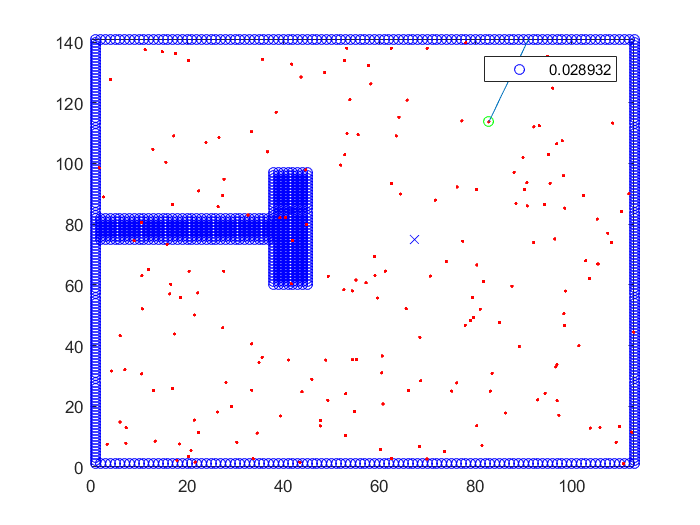
\includegraphics[width=.8\linewidth]{billeder/Results/1.png}
  \caption{Step 1}
  \label{ResultDriveFig1:sub1}
\end{subfigure}%
\begin{subfigure}{.5\textwidth}
  \centering
  \includegraphics[width=.7\linewidth]{billeder/Results/real1.png}
  \caption{Step 1}
  \label{ResultDriveFig1:sub2}
\end{subfigure}
\begin{subfigure}{.5\textwidth}
  \centering
  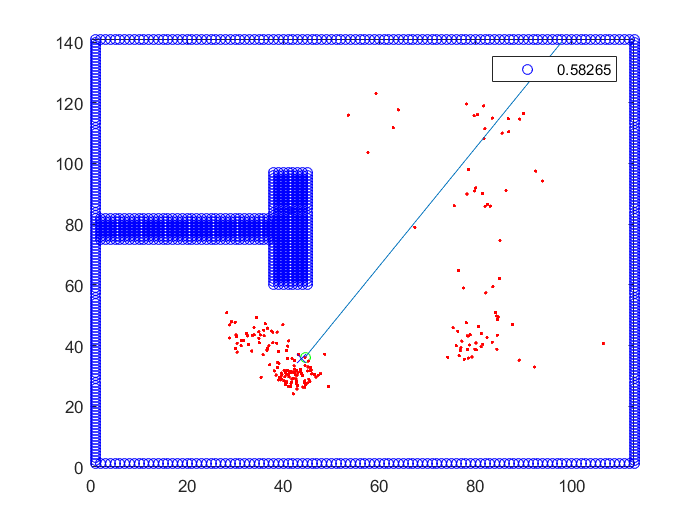
\includegraphics[width=.8\linewidth]{billeder/Results/3.png}
  \caption{Step 3}
  \label{ResultDriveFig1:sub3}
\end{subfigure}%
\begin{subfigure}{.5\textwidth}
  \centering
  \includegraphics[width=.7\linewidth]{billeder/Results/real3.png}
  \caption{Step 3}
  \label{ResultDriveFig1:sub4}
\end{subfigure}
\begin{subfigure}{.5\textwidth}
  \centering
  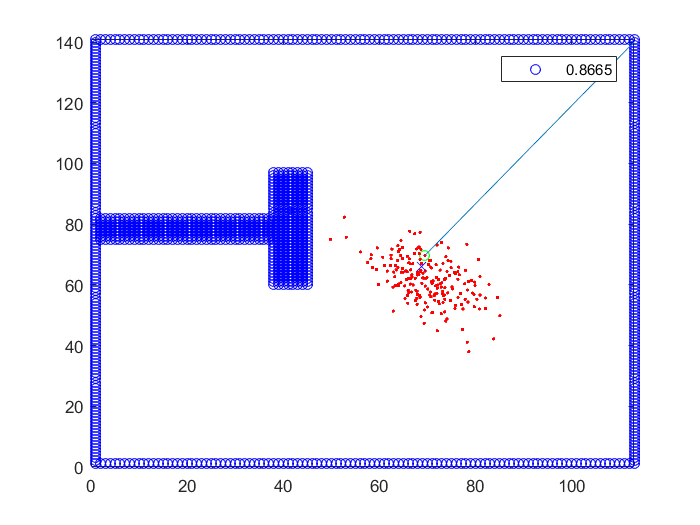
\includegraphics[width=.8\linewidth]{billeder/Results/5.png}
  \caption{Step 5}
  \label{ResultDriveFig1:sub5}
\end{subfigure}%
\begin{subfigure}{.5\textwidth}
  \centering
  \includegraphics[width=.7\linewidth]{billeder/Results/real5.png}
  \caption{Step 5}
  \label{ResultDriveFig1:sub6}
\end{subfigure}
\caption{The robot tries to find its location.}
\label{ResultDriveFig1}
\end{figure}
Figure \ref{ResultDriveFig2} shows the robot trying to make it towards the points of the plan. The point the robot is aiming for is marked by a blue '+' on the particle filter map. The robot has to be within  5 cm of the point to believe that it is in the correct position.
\begin{figure}[H]
\centering
\begin{subfigure}{.5\textwidth}
  \centering
  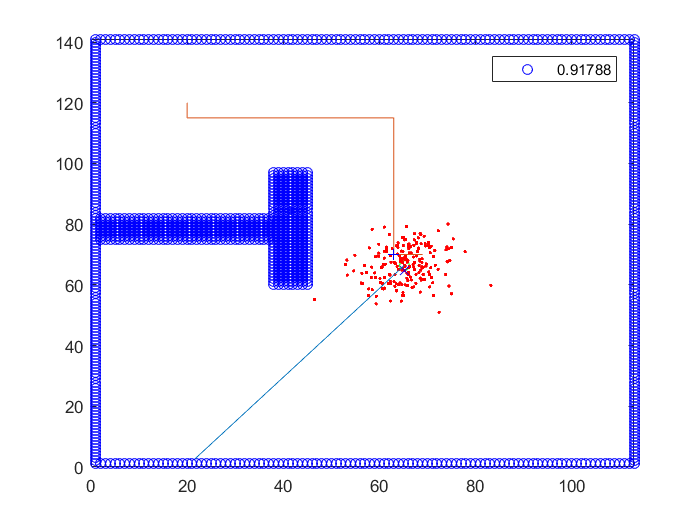
\includegraphics[width=.8\linewidth]{billeder/Results/7.png}
  \caption{Step 7}
  \label{ResultDriveFig2:sub1}
\end{subfigure}%
\begin{subfigure}{.5\textwidth}
  \centering
  \includegraphics[width=.7\linewidth]{billeder/Results/real7.png}
  \caption{Step 7}
  \label{ResultDriveFig2:sub2}
\end{subfigure}
\begin{subfigure}{.5\textwidth}
  \centering
  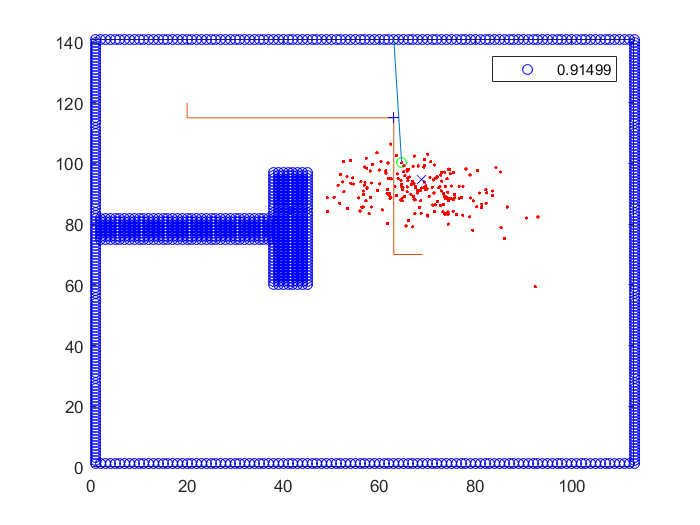
\includegraphics[width=.8\linewidth]{billeder/Results/9.png}
  \caption{Step 9}
  \label{ResultDriveFig2:sub3}
\end{subfigure}%
\begin{subfigure}{.5\textwidth}
  \centering
  \includegraphics[width=.7\linewidth]{billeder/Results/real9.png}
  \caption{Step 9}
  \label{ResultDriveFig2:sub4}
\end{subfigure}
\begin{subfigure}{.5\textwidth}
  \centering
  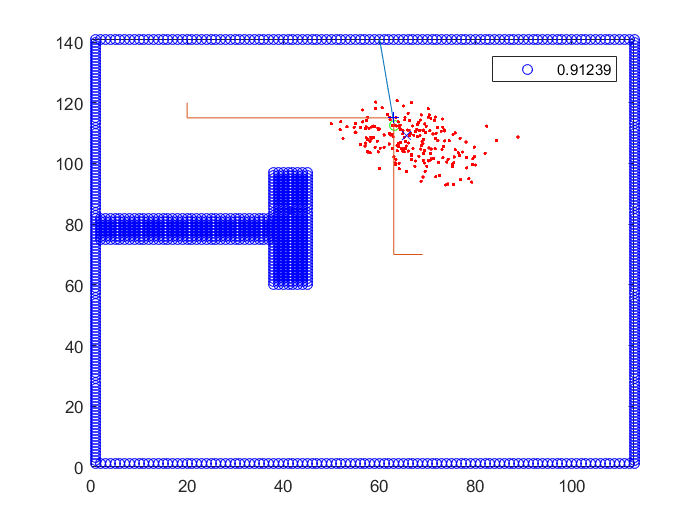
\includegraphics[width=.8\linewidth]{billeder/Results/11.png}
  \caption{Step 11}
  \label{ResultDriveFig2:sub5}
\end{subfigure}%
\begin{subfigure}{.5\textwidth}
  \centering
  \includegraphics[width=.7\linewidth]{billeder/Results/real11.png}
  \caption{Step 11}
  \label{ResultDriveFig2:sub6}
\end{subfigure}
\caption{The robot makes a map and moves along the points on the path.}
\label{ResultDriveFig2}
\end{figure}

\begin{figure}[H]
\centering
\begin{subfigure}{.5\textwidth}
  \centering
  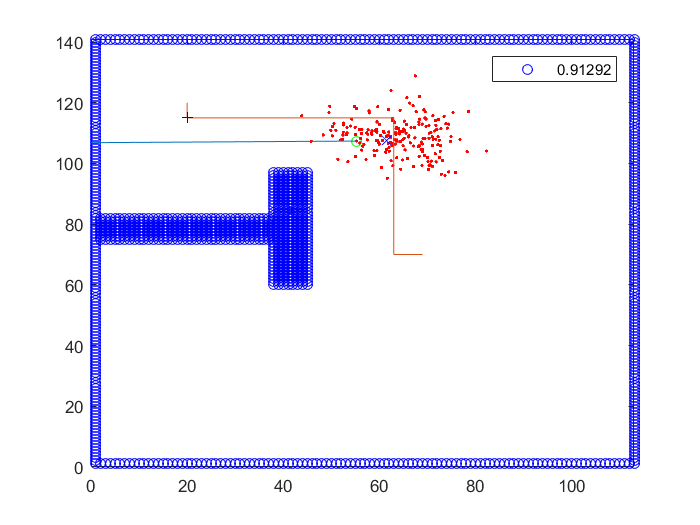
\includegraphics[width=.8\linewidth]{billeder/Results/13.png}
  \caption{Step 13}
  \label{ResultDriveFig3:sub1}
\end{subfigure}%
\begin{subfigure}{.5\textwidth}
  \centering
  \includegraphics[width=.7\linewidth]{billeder/Results/real13.png}
  \caption{Step 13}
  \label{ResultDriveFig3:sub2}
\end{subfigure}
\begin{subfigure}{.5\textwidth}
  \centering
  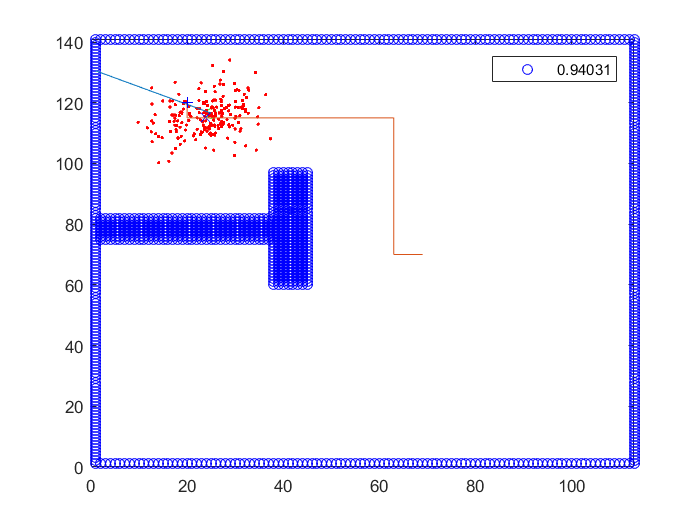
\includegraphics[width=.8\linewidth]{billeder/Results/19.png}
  \caption{Step 19}
  \label{ResultDriveFig3:sub3}
\end{subfigure}%
\begin{subfigure}{.5\textwidth}
  \centering
  \includegraphics[width=.7\linewidth]{billeder/Results/real19.png}
  \caption{Step 19}
  \label{ResultDriveFig3:sub4}
\end{subfigure}
\begin{subfigure}{.5\textwidth}
  \centering
  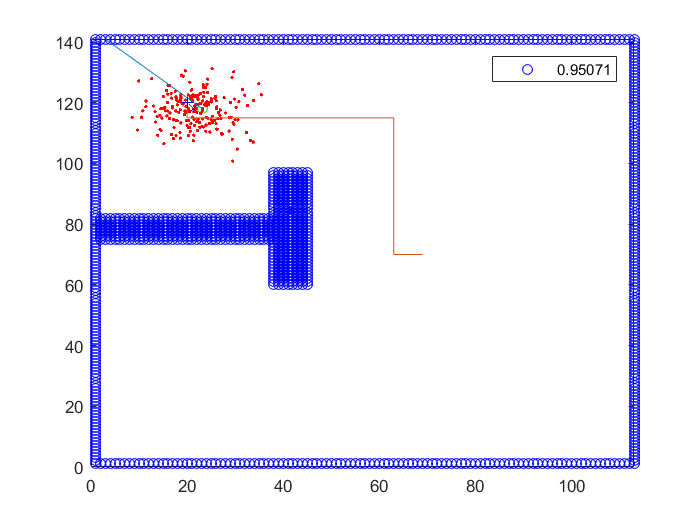
\includegraphics[width=.8\linewidth]{billeder/Results/23.png}
  \caption{Step 23}
  \label{ResultDriveFig3:sub5}
\end{subfigure}%
\begin{subfigure}{.5\textwidth}
  \centering
  \includegraphics[width=.7\linewidth]{billeder/Results/real23.png}
  \caption{Step 23}
  \label{ResultDriveFig3:sub6}
\end{subfigure}
\caption{The robot moves along the last points of the path and reaches goal.}
\label{ResultDriveFig3}
\end{figure}

The robot used 3 steps to find it self and in total it took 23 steps from beginning to end. 

%------------------------------------------------
\chapter{Discussion}
The motors were not fitted with tachometers which meant there was no way of getting reliable information about the wheels movement. This made it hard to determine the distance driven and the drift to either side. As a direct consequence of this, PID control and path smoothing was not used as the implementation of the PID controller would have been very complex and only relying on measurements from the LIDAR sensor. It was chosen that the PID controller implementation was out of the scope of this project. \\
To try to correct some of the movement noise the LIDAR data was used to inform of the actual movement. This worked fairly well for us. If we had more time one interesting experiment would be to use a Kalman filter to fuse the measurement from the LIDAR with the time based control input to get a even better estimate.

When a path plan is made, the plan is made from single centimetre steps into a  few coordinate sets. 
This is done because the robot has a hard time following the line and because of the lack of information from the wheels. 
When the robot is sufficiently close to one of the coordinate points, it will turn and head towards the next.
From the result it can be seen that the robot uses a lot of steps to achieve its goal after the correct path is found. 
This is mainly because the robot is not very certain of its own position, since most steps happens when it tries to get close to the point.

Another problem that was often seen during the previous testing, was that the robot drifted to one side. This was somewhat solved by giving one motor a slightly higher speed than the other. The drifting error became higher the longer the robot drove in one step. Therefore the maximal distance to drive was also set to 30 cm. This gives the robot a higher precision in movements, but it also results in more movements when longer routes are planned.\\
The Move forward function was not corrected the same way as the Turn function was. If it was corrected directly by reversing, if the robot drove too far, some of the overshoots may have been avoided.

When using the particle filter it is important to set the noise values corrected to get a optimal filter. In our filter the noise settings was good for finding the area where the true location was with relative few particles. But the noise settings prevented us for tuning in on the true location, by decreasing the area. This could be achieved by changing the noise as a function of the certainty.   
Another important aspect to consider when working with particle filters is the number of particles to be used. For a large map many particles is needed. The more particles the greater the calculation cost. It is therefore sometimes better to decrease the number of particles when the location have been found, since the very large amount is only truly needed in the initial location state. The optimal number is dependent of the application.

Some considerations shall also be made in regards to the re-sample time. In our implementation we re-sampled after every move. But for some applications it is a better strategy to make a series of moves and see how the probability of the particles is over time and re-sample based on this information. It is shown when comparing our results to results made by a other group, that this strategy preforms better in situations with many symmetric locations. This is since the re-sample operation is way more costly than the move operation. When doing a series of movements the chance of leaving the symmetric area before a re-sampling increases. 


\chapter{Conclusion}


%----------------------------------------------------------------------------------------
%	REFERENCE LIST
%----------------------------------------------------------------------------------------

\begin{thebibliography}{99} % Bibliography - this is intentionally simple in this template

\bibitem[Figueredo and Wolf, 2009]{Figueredo:2009dg}
Figueredo, A.~J. and Wolf, P. S.~A. (2009).
\newblock Assortative pairing and life history strategy - a cross-cultural
  study.
\newblock {\em Human Nature}, 20:317--330.
 
\end{thebibliography}

%----------------------------------------------------------------------------------------

%\end{multicols}

\end{document}